\documentclass{beamer}
\setbeamertemplate{caption}[numbered]
\usepackage{tikz}
\usepackage{graphicx}
\usetheme{AnnArbor}
%\usecolortheme{wolverine}
\title[AD for POMPs]{Automatic Differentiation Accelerates Inference for Partially Observed Stochastic Processes}
\subtitle{\small{Inference for Partially Observed Structured Dynamic Systems}}
\author[Kevin Tan]{Kevin Tan \\ \small{University of Pennsylvania, Department of Statistics and Data Science} \\\vspace{0.5cm} \small{Joint work with Giles Hooker and Edward Ionides}}
\date[January 4, 2024]{IMS Asia Pacific Rim Meeting \\ January 4, 2024}

\usepackage{amsmath}
\usepackage{tabularx}
\usepackage{mathtools}
\usepackage{bbold}
\usepackage[utf8]{inputenc} % allow utf-8 input
\usepackage[T1]{fontenc}    % use 8-bit T1 fonts
\usepackage{pifont}
%\usepackage[left=1in,right=1in,]{geometry}
\usepackage{multicol,lipsum,xcolor}
\usepackage{hyperref}       % hyperlinks
\usepackage{url}            % simple URL typesetting
\usepackage{amsmath,amsthm,amssymb,bm}
\usepackage{bbold}
\usepackage{caption}
\usepackage{graphicx}
\usepackage{enumerate}
%\usepackage{enumitem}
\usepackage{natbib}
\usepackage{parskip}
\usepackage{comment}
\usepackage{microtype}
\usepackage{diagbox}
\usepackage{tikz}
\usepackage{fancyhdr}
\usepackage{appendixnumberbeamer}


\newcommand{\Prob}{\displaystyle \mathbb {P}}
\newcommand{\jac}{\bigg| \frac{\dif x}{\dif y} \bigg|}
\newcommand{\inftyint}{\int_{-\infty}^{\infty}}
\newcommand{\X}{\mathcal{X}}
\newcommand{\Y}{\mathcal{Y}}
\newcommand{\N}{\mathbb{N}}
\newcommand{\Z}{\mathbb{Z}}
\newcommand{\C}{\mathbb{C}}

% best package ever
%\usepackage{realhats}

\def\mathfamilydefault{\rmdefault}

\usepackage{color}
\usepackage{xcolor}
\definecolor{hlpink}{rgb}{0.96, 0.76, 0.76}
\definecolor{hlblue}{rgb}{0.54, 0.81, 0.94}
\definecolor{hlyellow}{rgb}{0.98, 0.91, 0.71}
\definecolor{hlgreen}{rgb}{0.7, 0.93, 0.36}
\definecolor{hlpurple}{rgb}{0.8, 0.8, 1.0}

\newcommand{\highlight}[2][yellow]{\mathchoice%
  {\colorbox{#1}{$\displaystyle#2$}}%
  {\colorbox{#1}{$\textstyle#2$}}%
  {\colorbox{#1}{$\scriptstyle#2$}}%
  {\colorbox{#1}{$\scriptscriptstyle#2$}}}%
  
 \AtBeginSection[]{
  \begin{frame}
  \vfill
  \centering
  \begin{beamercolorbox}[sep=8pt,center,shadow=true,rounded=true]{title}
    \usebeamerfont{title}\insertsectionhead\par%
  \end{beamercolorbox}
  \vfill
  \end{frame}
}


%%%%% NEW MATH DEFINITIONS %%%%%
\usepackage{amsmath,bbm,bm}
\usepackage{amsfonts}
\usepackage{amsthm}
\usepackage{mathtools}

% algorithm
\usepackage{algorithm, algorithmic}
\usepackage{tabularx}
%\usepackage[table,xcdraw]{xcolor}
\usepackage{xcolor}
% commands
% global count (no section number)
\newtheorem{thm}{Theorem}%[section]
\newtheorem{lem}{Lemma}
\newtheorem{prop}{Proposition}
\newtheorem{cor}{Corollary}
\newtheorem{conj}{Conjecture}
\newtheorem{aspt}{Assumption}
\newtheorem{claim}{Claim}
\newtheorem{rmk}{Remark}
\newtheorem{commt}{Comment}
\newtheorem{defn}{Definition}

% Comments
% \usepackage{xcolor} % already loaded
\newcount\comments  % 0 suppresses notes to selves in text
\comments=0  % TODO: change to 0 for final version
\newcommand{\genComment}[2]{\ifnum\comments=1{\textcolor{#1}{\textsf{\footnotesize #2}}}\fi}
\newcommand{\ed}[1]{\genComment{red}{[EI:#1]}}
\newcommand{\giles}[1]{\genComment{green}{[GH:#1]}}
\newcommand{\kevin}[1]{\genComment{blue}{[KT:#1]}}

% Mark sections of captions for referring to divisions of figures
\newcommand{\figleft}{{\em (Left)}}
\newcommand{\figcenter}{{\em (Center)}}
\newcommand{\figright}{{\em (Right)}}
\newcommand{\figtop}{{\em (Top)}}
\newcommand{\figbottom}{{\em (Bottom)}}
\newcommand{\captiona}{{\em (a)}}
\newcommand{\captionb}{{\em (b)}}
\newcommand{\captionc}{{\em (c)}}
\newcommand{\captiond}{{\em (d)}}


\newcommand\seq[2]{{#1}\!:\!{#2}}
\newcommand\R{\mathbb{R}}
\newcommand\Var{\mathrm{Var}}
\newcommand\var{\Var}
\newcommand\Cov{\mathrm{Cov}}
\newcommand\cov{\Cov}
\newcommand\iid{\mathrm{iid}}
\newcommand\dist{d}
\newcommand\lik{\mathcal{L}}
\newcommand\prob{\mathbb{P}}
\newcommand\E{\mathbb{E}}
\newcommand\loglik{\ell}
\newcommand\process{\texttt{process}}
\newcommand\dimtheta{\mathrm{dim}_{\Theta}}
\newcommand\param{\,;}
\newcommand\giventh\param
\newcommand\given{{\,\vert\,}}
\newcommand\code[1]{\texttt{#1}}

\renewcommand\time{n}
\newcommand\myvec[1]{\boldsymbol{#1}}
\newcommand\altTime{\tilde n}
\newcommand\Time{N}
\newcommand\Np{J}
\newcommand\np{j}
\newcommand\altNp{k}
\newcommand\altAltNp{\tilde j}
\newcommand\resampleIndex{r}

% color
\newcommand{\blue}[1]{\textcolor{blue}{#1}}
\newcommand{\red}[1]{\textcolor{red}{#1}}
\newcommand{\orange}[1]{\textcolor{orange}{#1}}
\newcommand{\green}[1]{\textcolor{green}{#1}}

% Highlight a newly defined term
\newcommand{\newterm}[1]{{\bf #1}}


% Figure reference, lower-case.
\def\figref#1{figure~\ref{#1}}
% Figure reference, capital. For start of sentence
\def\Figref#1{Figure~\ref{#1}}
\def\twofigref#1#2{figures \ref{#1} and \ref{#2}}
\def\quadfigref#1#2#3#4{figures \ref{#1}, \ref{#2}, \ref{#3} and \ref{#4}}
% Section reference, lower-case.
\def\secref#1{section~\ref{#1}}
% Section reference, capital.
\def\Secref#1{Section~\ref{#1}}
% Reference to two sections.
\def\twosecrefs#1#2{sections \ref{#1} and \ref{#2}}
% Reference to three sections.
\def\secrefs#1#2#3{sections \ref{#1}, \ref{#2} and \ref{#3}}
% Reference to an equation, lower-case.
\def\eqref#1{equation~\ref{#1}}
% Reference to an equation, upper case
\def\Eqref#1{Equation~\ref{#1}}
% A raw reference to an equation---avoid using if possible
\def\plaineqref#1{\ref{#1}}
% Reference to a chapter, lower-case.
\def\chapref#1{chapter~\ref{#1}}
% Reference to an equation, upper case.
\def\Chapref#1{Chapter~\ref{#1}}
% Reference to a range of chapters
\def\rangechapref#1#2{chapters\ref{#1}--\ref{#2}}
% Reference to an algorithm, lower-case.
\def\algref#1{algorithm~\ref{#1}}
% Reference to an algorithm, upper case.
\def\Algref#1{Algorithm~\ref{#1}}
\def\twoalgref#1#2{algorithms \ref{#1} and \ref{#2}}
\def\Twoalgref#1#2{Algorithms \ref{#1} and \ref{#2}}
% Reference to a part, lower case
\def\partref#1{part~\ref{#1}}
% Reference to a part, upper case
\def\Partref#1{Part~\ref{#1}}
\def\twopartref#1#2{parts \ref{#1} and \ref{#2}}

\def\ceil#1{\lceil #1 \rceil}
\def\floor#1{\lfloor #1 \rfloor}
\def\1{\bm{1}}
\newcommand{\train}{\mathcal{D}}
\newcommand{\valid}{\mathcal{D_{\mathrm{valid}}}}
\newcommand{\test}{\mathcal{D_{\mathrm{test}}}}

\def\eps{{\epsilon}}


% Random variables
\def\reta{{\textnormal{$\eta$}}}
\def\ra{{\textnormal{a}}}
\def\rb{{\textnormal{b}}}
\def\rc{{\textnormal{c}}}
\def\rd{{\textnormal{d}}}
\def\re{{\textnormal{e}}}
\def\rf{{\textnormal{f}}}
\def\rg{{\textnormal{g}}}
\def\rh{{\textnormal{h}}}
\def\ri{{\textnormal{i}}}
\def\rj{{\textnormal{j}}}
\def\rk{{\textnormal{k}}}
\def\rl{{\textnormal{l}}}
% rm is already a command, just don't name any random variables m
\def\rn{{\textnormal{n}}}
\def\ro{{\textnormal{o}}}
\def\rp{{\textnormal{p}}}
\def\rq{{\textnormal{q}}}
\def\rr{{\textnormal{r}}}
\def\rs{{\textnormal{s}}}
\def\rt{{\textnormal{t}}}
\def\ru{{\textnormal{u}}}
\def\rv{{\textnormal{v}}}
\def\rw{{\textnormal{w}}}
\def\rx{{\textnormal{x}}}
\def\ry{{\textnormal{y}}}
\def\rz{{\textnormal{z}}}

% Random vectors
\def\rvepsilon{{\mathbf{\epsilon}}}
\def\rvtheta{{\mathbf{\theta}}}
\def\rva{{\mathbf{a}}}
\def\rvb{{\mathbf{b}}}
\def\rvc{{\mathbf{c}}}
\def\rvd{{\mathbf{d}}}
\def\rve{{\mathbf{e}}}
\def\rvf{{\mathbf{f}}}
\def\rvg{{\mathbf{g}}}
\def\rvh{{\mathbf{h}}}
\def\rvu{{\mathbf{i}}}
\def\rvj{{\mathbf{j}}}
\def\rvk{{\mathbf{k}}}
\def\rvl{{\mathbf{l}}}
\def\rvm{{\mathbf{m}}}
\def\rvn{{\mathbf{n}}}
\def\rvo{{\mathbf{o}}}
\def\rvp{{\mathbf{p}}}
\def\rvq{{\mathbf{q}}}
\def\rvr{{\mathbf{r}}}
\def\rvs{{\mathbf{s}}}
\def\rvt{{\mathbf{t}}}
\def\rvu{{\mathbf{u}}}
\def\rvv{{\mathbf{v}}}
\def\rvw{{\mathbf{w}}}
\def\rvx{{\mathbf{x}}}
\def\rvy{{\mathbf{y}}}
\def\rvz{{\mathbf{z}}}

% Elements of random vectors
\def\erva{{\textnormal{a}}}
\def\ervb{{\textnormal{b}}}
\def\ervc{{\textnormal{c}}}
\def\ervd{{\textnormal{d}}}
\def\erve{{\textnormal{e}}}
\def\ervf{{\textnormal{f}}}
\def\ervg{{\textnormal{g}}}
\def\ervh{{\textnormal{h}}}
\def\ervi{{\textnormal{i}}}
\def\ervj{{\textnormal{j}}}
\def\ervk{{\textnormal{k}}}
\def\ervl{{\textnormal{l}}}
\def\ervm{{\textnormal{m}}}
\def\ervn{{\textnormal{n}}}
\def\ervo{{\textnormal{o}}}
\def\ervp{{\textnormal{p}}}
\def\ervq{{\textnormal{q}}}
\def\ervr{{\textnormal{r}}}
\def\ervs{{\textnormal{s}}}
\def\ervt{{\textnormal{t}}}
\def\ervu{{\textnormal{u}}}
\def\ervv{{\textnormal{v}}}
\def\ervw{{\textnormal{w}}}
\def\ervx{{\textnormal{x}}}
\def\ervy{{\textnormal{y}}}
\def\ervz{{\textnormal{z}}}

% Random matrices
\def\rmA{{\mathbf{A}}}
\def\rmB{{\mathbf{B}}}
\def\rmC{{\mathbf{C}}}
\def\rmD{{\mathbf{D}}}
\def\rmE{{\mathbf{E}}}
\def\rmF{{\mathbf{F}}}
\def\rmG{{\mathbf{G}}}
\def\rmH{{\mathbf{H}}}
\def\rmI{{\mathbf{I}}}
\def\rmJ{{\mathbf{J}}}
\def\rmK{{\mathbf{K}}}
\def\rmL{{\mathbf{L}}}
\def\rmM{{\mathbf{M}}}
\def\rmN{{\mathbf{N}}}
\def\rmO{{\mathbf{O}}}
\def\rmP{{\mathbf{P}}}
\def\rmQ{{\mathbf{Q}}}
\def\rmR{{\mathbf{R}}}
\def\rmS{{\mathbf{S}}}
\def\rmT{{\mathbf{T}}}
\def\rmU{{\mathbf{U}}}
\def\rmV{{\mathbf{V}}}
\def\rmW{{\mathbf{W}}}
\def\rmX{{\mathbf{X}}}
\def\rmY{{\mathbf{Y}}}
\def\rmZ{{\mathbf{Z}}}

% Elements of random matrices
\def\ermA{{\textnormal{A}}}
\def\ermB{{\textnormal{B}}}
\def\ermC{{\textnormal{C}}}
\def\ermD{{\textnormal{D}}}
\def\ermE{{\textnormal{E}}}
\def\ermF{{\textnormal{F}}}
\def\ermG{{\textnormal{G}}}
\def\ermH{{\textnormal{H}}}
\def\ermI{{\textnormal{I}}}
\def\ermJ{{\textnormal{J}}}
\def\ermK{{\textnormal{K}}}
\def\ermL{{\textnormal{L}}}
\def\ermM{{\textnormal{M}}}
\def\ermN{{\textnormal{N}}}
\def\ermO{{\textnormal{O}}}
\def\ermP{{\textnormal{P}}}
\def\ermQ{{\textnormal{Q}}}
\def\ermR{{\textnormal{R}}}
\def\ermS{{\textnormal{S}}}
\def\ermT{{\textnormal{T}}}
\def\ermU{{\textnormal{U}}}
\def\ermV{{\textnormal{V}}}
\def\ermW{{\textnormal{W}}}
\def\ermX{{\textnormal{X}}}
\def\ermY{{\textnormal{Y}}}
\def\ermZ{{\textnormal{Z}}}

% Vectors
\def\vzero{{\bm{0}}}
\def\vone{{\bm{1}}}
\def\vmu{{\bm{\mu}}}
\def\vtheta{{\bm{\theta}}}
\def\va{{\bm{a}}}
\def\vb{{\bm{b}}}
\def\vc{{\bm{c}}}
\def\vd{{\bm{d}}}
\def\ve{{\bm{e}}}
\def\vf{{\bm{f}}}
\def\vg{{\bm{g}}}
\def\vh{{\bm{h}}}
\def\vi{{\bm{i}}}
\def\vj{{\bm{j}}}
\def\vk{{\bm{k}}}
\def\vl{{\bm{l}}}
\def\vm{{\bm{m}}}
\def\vn{{\bm{n}}}
\def\vo{{\bm{o}}}
\def\vp{{\bm{p}}}
\def\vq{{\bm{q}}}
\def\vr{{\bm{r}}}
\def\vs{{\bm{s}}}
\def\vt{{\bm{t}}}
\def\vu{{\bm{u}}}
\def\vv{{\bm{v}}}
\def\vw{{\bm{w}}}
\def\vx{{\bm{x}}}
\def\vy{{\bm{y}}}
\def\vz{{\bm{z}}}

% Elements of vectors
\def\evalpha{{\alpha}}
\def\evbeta{{\beta}}
\def\evepsilon{{\epsilon}}
\def\evlambda{{\lambda}}
\def\evomega{{\omega}}
\def\evmu{{\mu}}
\def\evpsi{{\psi}}
\def\evsigma{{\sigma}}
\def\evtheta{{\theta}}
\def\eva{{a}}
\def\evb{{b}}
\def\evc{{c}}
\def\evd{{d}}
\def\eve{{e}}
\def\evf{{f}}
\def\evg{{g}}
\def\evh{{h}}
\def\evi{{i}}
\def\evj{{j}}
\def\evk{{k}}
\def\evl{{l}}
\def\evm{{m}}
\def\evn{{n}}
\def\evo{{o}}
\def\evp{{p}}
\def\evq{{q}}
\def\evr{{r}}
\def\evs{{s}}
\def\evt{{t}}
\def\evu{{u}}
\def\evv{{v}}
\def\evw{{w}}
\def\evx{{x}}
\def\evy{{y}}
\def\evz{{z}}

% Matrix
\def\mA{{\bm{A}}}
\def\mB{{\bm{B}}}
\def\mC{{\bm{C}}}
\def\mD{{\bm{D}}}
\def\mE{{\bm{E}}}
\def\mF{{\bm{F}}}
\def\mG{{\bm{G}}}
\def\mH{{\bm{H}}}
\def\mI{{\bm{I}}}
\def\mJ{{\bm{J}}}
\def\mK{{\bm{K}}}
\def\mL{{\bm{L}}}
\def\mM{{\bm{M}}}
\def\mN{{\bm{N}}}
\def\mO{{\bm{O}}}
\def\mP{{\bm{P}}}
\def\mQ{{\bm{Q}}}
\def\mR{{\bm{R}}}
\def\mS{{\bm{S}}}
\def\mT{{\bm{T}}}
\def\mU{{\bm{U}}}
\def\mV{{\bm{V}}}
\def\mW{{\bm{W}}}
\def\mX{{\bm{X}}}
\def\mY{{\bm{Y}}}
\def\mZ{{\bm{Z}}}
\def\mBeta{{\bm{\beta}}}
\def\mPhi{{\bm{\Phi}}}
\def\mLambda{{\bm{\Lambda}}}
\def\mSigma{{\bm{\Sigma}}}

% Tensor
\DeclareMathAlphabet{\mathsfit}{\encodingdefault}{\sfdefault}{m}{sl}
\SetMathAlphabet{\mathsfit}{bold}{\encodingdefault}{\sfdefault}{bx}{n}
\newcommand{\tens}[1]{\bm{\mathsfit{#1}}}
\def\tA{{\tens{A}}}
\def\tB{{\tens{B}}}
\def\tC{{\tens{C}}}
\def\tD{{\tens{D}}}
\def\tE{{\tens{E}}}
\def\tF{{\tens{F}}}
\def\tG{{\tens{G}}}
\def\tH{{\tens{H}}}
\def\tI{{\tens{I}}}
\def\tJ{{\tens{J}}}
\def\tK{{\tens{K}}}
\def\tL{{\tens{L}}}
\def\tM{{\tens{M}}}
\def\tN{{\tens{N}}}
\def\tO{{\tens{O}}}
\def\tP{{\tens{P}}}
\def\tQ{{\tens{Q}}}
\def\tR{{\tens{R}}}
\def\tS{{\tens{S}}}
\def\tT{{\tens{T}}}
\def\tU{{\tens{U}}}
\def\tV{{\tens{V}}}
\def\tW{{\tens{W}}}
\def\tX{{\tens{X}}}
\def\tY{{\tens{Y}}}
\def\tZ{{\tens{Z}}}


% Graph
\def\gA{{\mathcal{A}}}
\def\gB{{\mathcal{B}}}
\def\gC{{\mathcal{C}}}
\def\gD{{\mathcal{D}}}
\def\gE{{\mathcal{E}}}
\def\gF{{\mathcal{F}}}
\def\gG{{\mathcal{G}}}
\def\gH{{\mathcal{H}}}
\def\gI{{\mathcal{I}}}
\def\gJ{{\mathcal{J}}}
\def\gK{{\mathcal{K}}}
\def\gL{{\mathcal{L}}}
\def\gM{{\mathcal{M}}}
\def\gN{{\mathcal{N}}}
\def\gO{{\mathcal{O}}}
\def\gP{{\mathcal{P}}}
\def\gQ{{\mathcal{Q}}}
\def\gR{{\mathcal{R}}}
\def\gS{{\mathcal{S}}}
\def\gT{{\mathcal{T}}}
\def\gU{{\mathcal{U}}}
\def\gV{{\mathcal{V}}}
\def\gW{{\mathcal{W}}}
\def\gX{{\mathcal{X}}}
\def\gY{{\mathcal{Y}}}
\def\gZ{{\mathcal{Z}}}

% Sets
\def\sA{{\mathbb{A}}}
\def\sB{{\mathbb{B}}}
\def\sC{{\mathbb{C}}}
\def\sD{{\mathbb{D}}}
% Don't use a set called E, because this would be the same as our symbol
% for expectation.
\def\sF{{\mathbb{F}}}
\def\sG{{\mathbb{G}}}
\def\sH{{\mathbb{H}}}
\def\sI{{\mathbb{I}}}
\def\sJ{{\mathbb{J}}}
\def\sK{{\mathbb{K}}}
\def\sL{{\mathbb{L}}}
\def\sM{{\mathbb{M}}}
\def\sN{{\mathbb{N}}}
\def\sO{{\mathbb{O}}}
\def\sP{{\mathbb{P}}}
\def\sQ{{\mathbb{Q}}}
\def\sR{{\mathbb{R}}}
\def\sS{{\mathbb{S}}}
\def\sT{{\mathbb{T}}}
\def\sU{{\mathbb{U}}}
\def\sV{{\mathbb{V}}}
\def\sW{{\mathbb{W}}}
\def\sX{{\mathbb{X}}}
\def\sY{{\mathbb{Y}}}
\def\sZ{{\mathbb{Z}}}

% Entries of a matrix
\def\emLambda{{\Lambda}}
\def\emA{{A}}
\def\emB{{B}}
\def\emC{{C}}
\def\emD{{D}}
\def\emE{{E}}
\def\emF{{F}}
\def\emG{{G}}
\def\emH{{H}}
\def\emI{{I}}
\def\emJ{{J}}
\def\emK{{K}}
\def\emL{{L}}
\def\emM{{M}}
\def\emN{{N}}
\def\emO{{O}}
\def\emP{{P}}
\def\emQ{{Q}}
\def\emR{{R}}
\def\emS{{S}}
\def\emT{{T}}
\def\emU{{U}}
\def\emV{{V}}
\def\emW{{W}}
\def\emX{{X}}
\def\emY{{Y}}
\def\emZ{{Z}}
\def\emSigma{{\Sigma}}

% entries of a tensor
% Same font as tensor, without \bm wrapper
\newcommand{\etens}[1]{\mathsfit{#1}}
\def\etLambda{{\etens{\Lambda}}}
\def\etA{{\etens{A}}}
\def\etB{{\etens{B}}}
\def\etC{{\etens{C}}}
\def\etD{{\etens{D}}}
\def\etE{{\etens{E}}}
\def\etF{{\etens{F}}}
\def\etG{{\etens{G}}}
\def\etH{{\etens{H}}}
\def\etI{{\etens{I}}}
\def\etJ{{\etens{J}}}
\def\etK{{\etens{K}}}
\def\etL{{\etens{L}}}
\def\etM{{\etens{M}}}
\def\etN{{\etens{N}}}
\def\etO{{\etens{O}}}
\def\etP{{\etens{P}}}
\def\etQ{{\etens{Q}}}
\def\etR{{\etens{R}}}
\def\etS{{\etens{S}}}
\def\etT{{\etens{T}}}
\def\etU{{\etens{U}}}
\def\etV{{\etens{V}}}
\def\etW{{\etens{W}}}
\def\etX{{\etens{X}}}
\def\etY{{\etens{Y}}}
\def\etZ{{\etens{Z}}}

% The true underlying data generating distribution
\newcommand{\pdata}{p_{\rm{data}}}
% The empirical distribution defined by the training set
\newcommand{\ptrain}{\hat{p}_{\rm{data}}}
\newcommand{\Ptrain}{\hat{P}_{\rm{data}}}
% The model distribution
\newcommand{\pmodel}{p_{\rm{model}}}
\newcommand{\Pmodel}{P_{\rm{model}}}
\newcommand{\ptildemodel}{\tilde{p}_{\rm{model}}}
% Stochastic autoencoder distributions
\newcommand{\pencode}{p_{\rm{encoder}}}
\newcommand{\pdecode}{p_{\rm{decoder}}}
\newcommand{\precons}{p_{\rm{reconstruct}}}

\newcommand{\laplace}{\mathrm{Laplace}} % Laplace distribution

\newcommand{\Ls}{\mathcal{L}}
\newcommand{\emp}{\tilde{p}}
\newcommand{\lr}{\alpha}
\newcommand{\reg}{\lambda}
\newcommand{\rect}{\mathrm{rectifier}}
\newcommand{\softmax}{\mathrm{softmax}}
\newcommand{\sigmoid}{\sigma}
\newcommand{\softplus}{\zeta}
\newcommand{\KL}{D_{\mathrm{KL}}}
%\newcommand{\Var}{\mathrm{Var}}
\newcommand{\standarderror}{\mathrm{SE}}
%\newcommand{\Cov}{\mathrm{Cov}}
% Wolfram Mathworld says $L^2$ is for function spaces and $\ell^2$ is for vectors
% But then they seem to use $L^2$ for vectors throughout the site, and so does
% wikipedia.
\newcommand{\normlzero}{L^0}
\newcommand{\normlone}{L^1}
\newcommand{\normltwo}{L^2}
\newcommand{\normlp}{L^p}
\newcommand{\normmax}{L^\infty}

\newcommand{\parents}{Pa} % See usage in notation.tex. Chosen to match Daphne's book.

\let\ab\allowbreak

  
\begin{document}



\maketitle


\section{Background}


\begin{frame}{Partially Observed Markov Processes}

    \begin{itemize}
        \item Unobserved Markov process $\{X_t, t \geq t_0\}$, observations $y_1^*,...,y_N^*$ at timesteps $t_1,..., t_N$.
        \item \pause Unknown parameter $\theta \in \Theta$, to be estimated.
        \item \textbf{Notation:}
        \begin{itemize}
            \item $f_{X_n|X_{n-1}}\left(x_{n} \mid x_{n-1}; \theta\right)$ is the \textbf{process model}.
            \item \pause $\texttt{process}\left(x_n, \theta\right)$ is the \textbf{simulator} corresponding to the process model. 
            \item \pause $f_{Y_n|X_n}\left(y_n \mid x_n, \theta\right)$ is the \textbf{measurement model}.
        \end{itemize}
    \end{itemize}
\end{frame}


\begin{frame}{Particle Filters}

    \begin{figure}
        \centering
        \begin{minipage}[c]{0.5\textwidth}
            \centering
            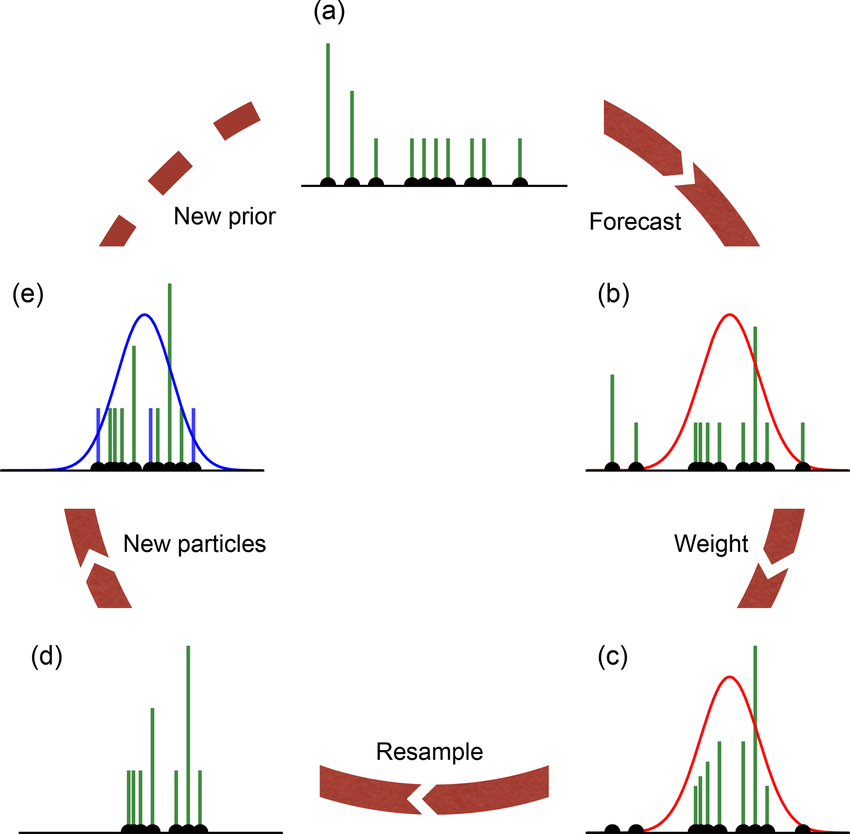
\includegraphics[scale=0.15]{imgs/pfilter.png}
            \end{minipage}
        \begin{minipage}[c]{0.45\textwidth}
            \caption{
            \\
            -- Dirac measure approximation of the Bayes filter. 
            \\ 
            -- Yields a filtering distribution and likelihood estimate.
            \\ 
            -- Graphic from \cite{berg2019pfilterimage}.}
        \end{minipage}
        \label{fig:pfilter-illustration}
    \end{figure}
    
    \begin{itemize}
        \item Monte Carlo approximation of the Bayes filter.
        \begin{itemize}
            \item \pause Maintain belief on current state $x_n^F$. 
            \item \pause Simulate forward to get $x_{n+1}^P$, observe observation $y_{n+1}^*$.
            \item \pause Update $x_{n+1}^F$ accordingly.
        \end{itemize}
    \end{itemize}
\end{frame}


\begin{frame}{Automatic Differentiation}

    \begin{figure}
        \begin{minipage}[c]{0.7\textwidth}
            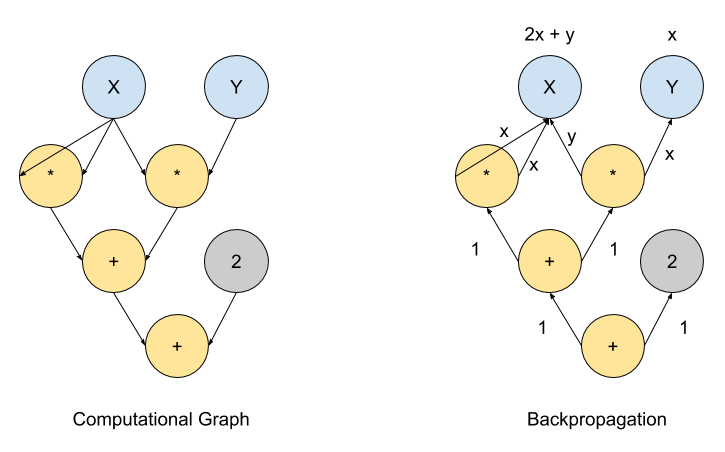
\includegraphics[scale=0.3]{imgs/autograd.png}
        \end{minipage}
        \begin{minipage}[l]{0.27\textwidth}
            \caption{
            \\$f(x,y) = x^2+xy+2$, $f'(x,y) = (2x+y,x).$
            -- Figure from \href{https://avinashselvam.medium.com/automatic-differentiation-explained-9f02c74e9a90}{Medium}.}
        \end{minipage}
        \label{fig:autograd-illustration}
    \end{figure}
    
    \begin{itemize}
        \item Evaluates the gradient of a (scalar or vector-valued) computer program w.r.t. its arguments.
        \item \pause Traverses computational graph (of primitive functions) with chain rule.
    \end{itemize}
    
\end{frame}


\section{Motivation}

\begin{frame}{Maximum Likelihood Inference is Hard in POMPs}
    
\begin{enumerate}
    \item \textbf{Intractable likelihood functions}! Bypassed with e.g. simulated likelihood, likelihood-free inference, particle filters, etc. 
    \item \pause May not have access to transition densities, only a \textbf{simulator}. 
    \begin{itemize}
        \item \pause IF2 (\cite{ionides15}), particle MCMC (\cite{doucet2010pmcmc}), only full-information methods that can deal with this.
    \end{itemize}
    \item \pause \textbf{Significant Monte-Carlo noise in likelihood estimate} makes accurate parameter estimation difficult.
\end{enumerate}
\end{frame}

\begin{frame}{IF2 Plateaus Quickly But Struggles to Find the MLE}
\begin{figure}
    \centering
    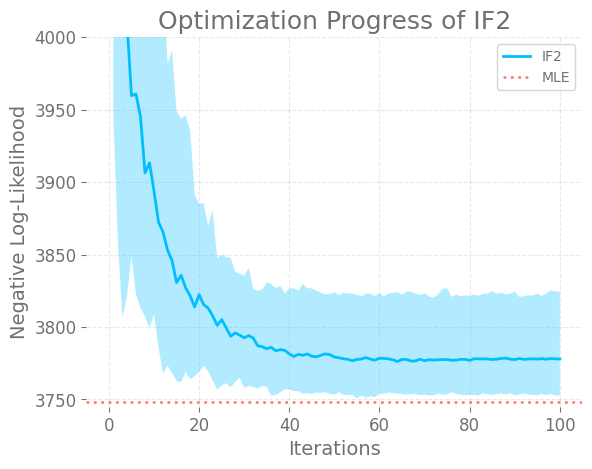
\includegraphics[scale=0.5]{imgs/095/if2fail.png}
    \caption{Performance of IF2 on \cite{king08} Dhaka cholera model. Shaded area represents 0th to 80th percentile, solid line is median of 100 runs. While IF2 makes quick initial progress, it fails to find the MLE.}
    \label{fig:if2fail}
\end{figure}
\end{frame}

\begin{frame}{Hang on, wait a minute!}
    \begin{itemize}
        \item Original iterated filtering algorithm: (noisy) approximation of score (\cite{ionides06-pnas}). 
        %\item \pause Performed a single "gradient step" at the end of each filtering iteration.
        \pause
        \item \textbf{Would performing automatic differentiation (AD) on the likelihood estimate from the particle filter lead to a less noisy score approximation?}
    \end{itemize}
    \pause
    \begin{block}{Problem!}
        But the particle filter has discrete stochastic resampling! How can we differentiate this?
    \end{block}
\end{frame}

\section{Previous Work: AD for Particle Filters}


\begin{frame}{Previous Work}

    \begin{table}[h!]
        \centering
        \begin{tabular}{||c c||} 
         \hline
         Authors & Method \\ [0.5ex] 
         \hline\hline
         \cite{poyiadjis11} & Particle approximation of score
         \\ & $O(N^2)$ variance, unbiased \\
         \hline
         \cite{blei2018vsmc} & Backprop through vanilla PF \\ 
         & Asymptotic bias \\
         \hline
         \cite{corenflos21} & Optimal transport resampling \\
         & Consistent, $O(J^2)$ runtime \\
         \hline
         \cite{scibior21} & Stop-gradient trick \\ 
         & Recovers \cite{poyiadjis11} with AD \\
         \hline 
         \cite{singh22} & Fixed-lag smoothing \\ 
         & Need transition densities \\ 
         \hline
        \end{tabular}
        \label{table:lit-review}
    \end{table}
\end{frame}


\begin{frame}{Our Contributions}
    \begin{itemize}
        \item New theoretical framework/algorithm/gradient estimator we call MOP-$\alpha$.
        \begin{itemize}
            \item \pause Gradient estimates of \cite{blei2018vsmc} (MOP-0), \cite{poyiadjis11} and \cite{scibior2021dpf} (MOP-1) are special cases.
            \item \pause Does not need transition densities, only a differentiable simulator.
            \item \pause Can optimize a bias-variance tradeoff. 
        \end{itemize}
        \item \pause Promising hybrid algorithm, warm-starts gradient descent (using this estimator) with IF2.
        \item \pause Outperforms IF2 on Cholera model of \cite{king08}.
    \end{itemize}
\end{frame}


\section{Smooth Extensions to the Particle Filter}

\begin{frame}{Intuition}
    \begin{block}{Problem}
        Want to differentiate through the particle filter. But the particle filter has discrete stochastic resampling! 
    \end{block}
    \pause 
    \begin{block}{Idea}
        Don't differentiate $\hat\ell(\theta)$ directly, differentiate through a (suitably) reweighted bootstrap filter.
    \end{block}
    \begin{itemize}
        \item \pause Particle filter run with state transitions \& resampling under $\phi \in \Theta$. 
        \item \pause Reweight to evaluate likelihood at nearby $\theta \in \Theta$ (same resampling).
        \item \pause Fix seed to treat particles, weights under $\phi$ as constants.
        \item \pause \textbf{Now only need to differentiate through likelihood ratios!}
    \end{itemize}
\end{frame}

\begin{frame}{What is this reweighting?}
    Ordinarily, the likelihood estimate for $\phi$ is 
    $$\hat\lik(\phi) = \prod_{n=1}^N \frac{1}{J} \sum_{j=1}^J \left(\underbrace{f_{Y_n|X_n}(y_n^* | x_{n,j}^{P,\phi}, \phi)}_{\textcolor{blue}{\text{Measurement Model}}}
    \cdot 
    \underbrace{f_{X_n|X_{n-1}}(x_{n,j}^{P, \phi} | x_{n-1,j}^{F,\phi}, \phi)}_{\textcolor{red}{\text{Process model}}}\right).$$
    \pause
    So to estimate the likelihood for $\theta$, we can correct 
    $$
        \hat\lik(\theta) 
        = \prod_{n=1}^N \frac{1}{J} \sum_{j=1}^J f_{Y_n|X_n}(y_n^* | x_{n,j}^{P,\phi}, \phi) \cdot 
        f_{X_n|X_{n-1}}(x_{n,j}^{P, \phi} | x_{n-1,j}^{F,\phi}, \phi) 
        \cdot \underbrace{s_{n,j} \cdot r_{n,j}}_{\text{Correction Term}},
    $$
    \pause
    where the multiplicative correction terms are
    $$
        \underbrace{s_{n,j}=\frac{g_{n,j}^\theta}{g_{n,j}^{\phi}}=\frac{f_{Y_n|X_n}(y_n^*|x_{n,j}^{P, \phi}; \theta)}{f_{Y_n|X_n}(y_n^*|x_{n,j}^{P,\phi}; \phi)}}_{\textcolor{blue}{\text{Measurement Model Likelihood Ratios}}},\;\; \underbrace{r_{n,j}=\frac{f_{X_n|X_{n-1}}(x_{n,j}^{P, \phi}|x_{n-1,j}^{F, \phi}; \theta)}{f_{X_n|X_{n-1}}(x_{n,j}^{P, \phi}|x_{n-1,j}^{F, \phi}; \phi)}}_{\textcolor{red}{\text{Process Model Likelihood Ratios}}}.
    $$
        
\end{frame}

\begin{frame}{New Problem}
    \begin{block}{Problem}
        Need likelihood ratios w.r.t. process and measurement models!
    \end{block}
    \pause 
    \begin{block}{Solution}
        Offload process model derivatives to differentiable simulator. 
    \end{block}
    \begin{itemize}
        \item \pause Run particle filter twice under same seed: one with process model at $\phi$, another with process model at $\theta$. Resample according to $\phi$.
        \item \pause Correct only with resampling likelihood ratios. 
        \item \pause Introduce additional discounting parameter $\alpha$ for bias-variance tradeoff.
    \end{itemize}
\end{frame}



\begin{frame}{Algorithm: Measurement Off-Policy, MOP-$\alpha$}
    \begin{enumerate}
        \item \textbf{Run a particle filter once at} $\phi$ to obtain $X_{n,j}^{P,\phi}, X_{n,j}^{F,\phi}$. Fix seed throughout. Set initial weights $w_{0,j}^{F,\theta} = 1/J$.
        \item \pause \textbf{At each timestep,} propagate weights $w_{n,j}^{P,\theta} := (w_{n-1,j}^{F,\theta})^\alpha$. 
        \item \pause Simulate process model ${X}_{n,j}^{P,\theta}\sim {f}_{{X}_{n}|{X}_{n-1}}\big(\cdot|{X}_{n-1,j}^{F};{\theta}\big)$, evaluate measurement model $g^{\theta}_{n,j}={f}_{{Y}_{n}|{X}_{n}}(y_{n}^{*}|{X}_{n,j}^{P,\theta}\giventh{\theta})$, evaluate conditional likelihood under $\phi$, $L_n^{\phi} = \frac{1}{J}\sum_{m=1}^{J}g^{\phi}_{n,m}$, \textbf{as usual.}
        \item \pause \textbf{Resample according to $\phi$:} $k_{1:J} \sim \prob\big(k_{j}=m\big) \propto g^{\phi}_{n,m}$.
        \item \pause \textbf{Correct filtering weights:} $\displaystyle w^{F,\theta}_{n,j}= w^{P,\theta}_{n,k_j} \times  g^{\theta}_{n,k_j}/ g^{\phi}_{n,k_j}$. 
    \end{enumerate}
    \pause 
    \centering{\textbf{Special Case:} If $\theta=\phi$, only need to run one particle filter! Set $X_{n,j}^{P,\theta}, X_{n,j}^{F,\theta}$ to be copies of the $\phi$ counterparts, where gradients don't propagate. Explains the \textbf{stop-gradient} trick of \cite{scibior21}.}
\end{frame}


\begin{frame}{Bias-Variance Tradeoff with $\alpha$}
\begin{itemize}
    \item $\alpha$ balances a tradeoff between:
    \begin{itemize}
        \item \pause Maintaining memory of each particle's ancestral trajectory (most extreme when $\alpha=1$).
        \item \pause Considering only the single-step transition dynamics (when $\alpha=0$).
    \end{itemize}
    \item \pause\textbf{Exponentially-weighted moving average} where $\alpha$ controls the amount of discounting.
    \item \pause Bias small if $y_{n+1:N}^*$ not informative for $x_n$ given $y_{0:n}^*$ (\cite{corenflos21}).
\end{itemize}
    
\end{frame}


\begin{frame}{Bias-Variance Tradeoff with $\alpha$}
\begin{figure}
    \centering
    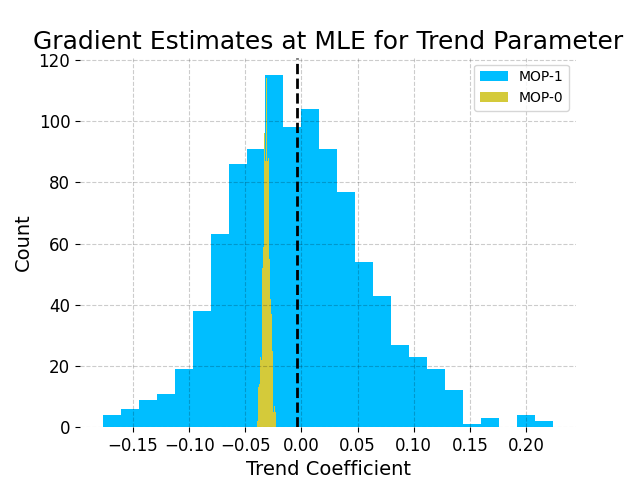
\includegraphics[scale=0.5]{imgs/mlegrad.png}
    \caption{Gradient estimates at MLE for trend in \cite{king08} cholera model. When $\alpha=1$, estimate close to unbiased with high variance. When $\alpha=0$, lower variance but biased.}
    \label{fig:bias-variance}
\end{figure}
    
\end{frame}

\begin{frame}{Bias-Variance Tradeoff with $\alpha$}
\begin{figure}
    \centering
    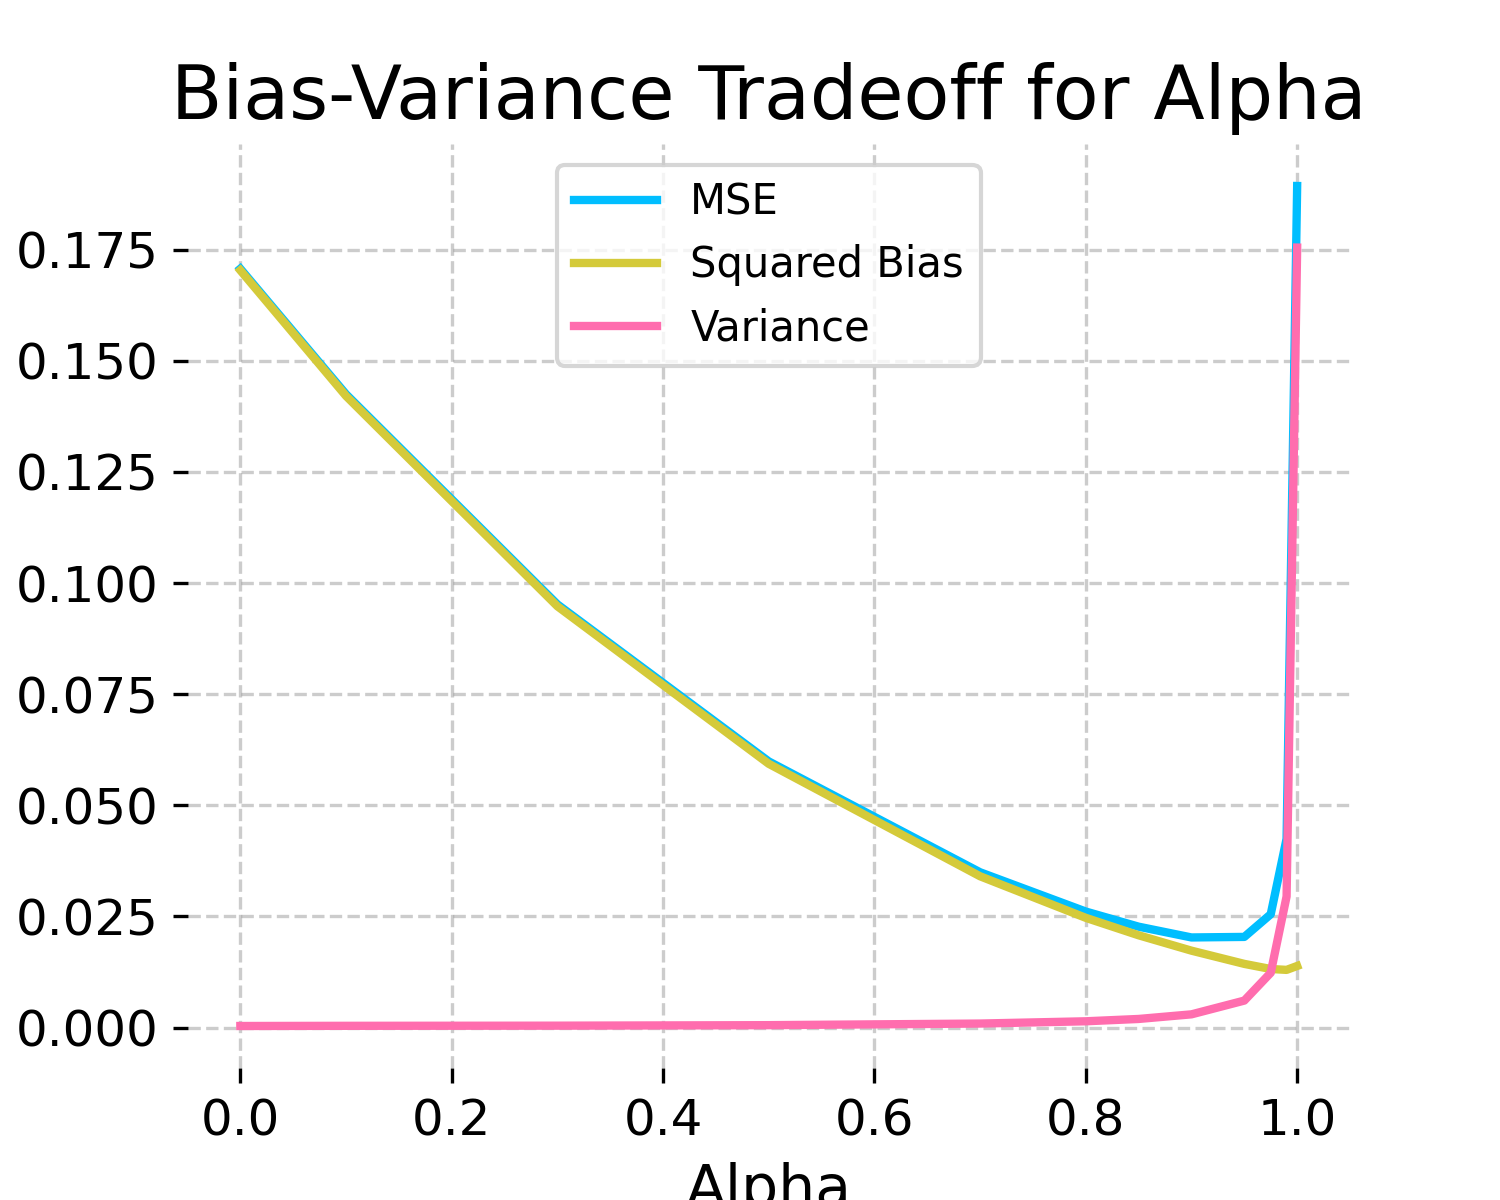
\includegraphics[scale=0.5]{imgs/095/biasvar.png}
    \caption{Bias-variance tradeoff for gradient estimates at MLE for trend in \cite{king08} cholera model. When $\alpha=1$, estimate close to unbiased with high variance. When $\alpha=0$, lower variance but biased. MSE seems to be minimized at $\alpha=0.97$.}
    \label{fig:bias-variance}
\end{figure}
    
\end{frame}

\begin{frame}{Guarantee}
    \begin{prop}[Correctness of MOP-$\alpha$]
    \label{prop:mop-correctness}
    When either $\alpha=1$ or $\theta=\phi$, MOP-$\alpha$ targets the posterior and is unbiased for the likelihood under $\theta$. 
    When $\theta$ is evaluated at $\phi$, the likelihood estimate agrees with the bootstrap filter. Its gradient when $\alpha=1$ is the estimate of \citet{poyiadjis11},
    $$\frac{1}{J}\sum_{j=1}^J \nabla_\theta \log f_{Y_{1:N}|X_{0:N}}(y_{1:N}^*|x_{1:N,j}^{A, F,\theta}),$$
    and when $\alpha=0,$ is the gradient estimator of \cite{blei2018vsmc},
    $$
        \frac{1}{J} \sum_{n=1}^N \sum_{j=1}^J \nabla_\theta \log f_{Y_n|X_{n}}(y_n^*|x_{n,j}^{F, \theta}; \theta),
    $$
    i.e. differentiating through a vanilla particle filter (\cite{scibior21}).
\end{prop}
\end{frame}



\section{Practical Maximum Likelihood Inference}

\begin{frame}{One possible procedure:}
    \begin{itemize}
        \item Warm-start gradient descent, or some other first or second order procedure (using the gradient estimate given by MOP-$\alpha$), with the output of an initial search of IF2. 
        \item \pause Run IF2, aggressively cooling to a fixed learning rate, till search stalls.
        \item \pause Refine this coarse solution with gradient descent.
    \end{itemize}
    \pause
    \centering{\textbf{Iterated Filtering with Automatic Differentiation (IFAD)}}
\end{frame}


\begin{frame}{Convergence Analysis}
    \begin{prop}[Convergence of IFAD-1]
        \label{thm:convergence}
        
        Consider a variant of IFAD-1 where one stops if the gradient estimate $||g(\theta_n)|| \leq \sigma \epsilon$. Assume $-\ell$ is $\gamma$-strongly convex, $\gamma I \preceq \nabla_\theta^2 (-\ell) \preceq \Gamma I$. $\sigma = \frac{4 \Gamma}{(1-\beta)}> 4$. Define $G$ as in Assumption \ref{assump:local-bounded-derivative}.
        
        Let $H(\theta_n)$ be a matrix possibly dependent on $\theta_n$ with minimum eigenvalue always greater than some $c>0$. Choose learning rate $\eta$ and error tolerance $\epsilon$ such that, where $\beta$ is the Armijo condition hyperparameter,
        \begin{equation*}
            \eta \leq \frac{c(1-\beta)}{\Gamma}, \;\; \epsilon \leq \frac{c(1-\beta)}{2\Gamma}||g(\theta_n)||.
        \end{equation*}
        
        Then, with $J$ large enough, the following holds with probability at least $1-\delta$:
        \begin{equation*}
        \ell(\theta^*) - \ell(\theta_{n+1}) \leq \left(1-\eta\beta\frac{8\gamma}{9c}\right)(\ell(\theta^*)-\ell(\theta_n))
        \end{equation*}
        
        and the algorithm terminates when $||\nabla_\theta \ell(\theta_n)|| \leq (1+\sigma) \epsilon$.
        \end{prop}
\end{frame}

\begin{frame}{Convergence Analysis}
    \begin{itemize}
        \item Similar to \cite{mahoney16}, uses concentration inequalities from \cite{delmoral2011ci}.
        \item Gradient stage of IFAD-1 converges linearly to the MLE if:
        \begin{enumerate}
            \item \pause The log-likelihood surface is $\gamma$-strongly convex in a neighborhood of the MLE.
            \item \pause The IF2 stage of IFAD successfully reaches a (high-probability) basin of attraction of the MLE. 
        \end{enumerate}
        \item \pause \textbf{Conjecture:} This applies to the entirety of IFAD, as IF2 converges very quickly to a neighborhood of the MLE and behaves a lot like SGD. 
    \end{itemize}
    
\end{frame}


\begin{frame}{Runtime}

\begin{itemize}
    \item Warm-start:
    \begin{itemize}
        \item \pause Initial warm-start "convergence" happens fairly quickly in practice. 
        \begin{itemize}
            \item \pause Dhaka cholera model of \cite{king08}: 40 iterations, usually 100-200 for global search.
        \end{itemize}
    \end{itemize}
    \item \pause MOP-$\alpha$:
    \begin{itemize}
        \item \pause Gradient takes 3.75x time of \texttt{pfilter()}, in line with cheap gradient principle (\cite{kakade2019provably}).
    \end{itemize}
    \item \pause Runtime \textbf{linear, and not quadratic}, in number of particles.
    \item \pause Re-implementation in \texttt{JAX} (\cite{jax2018github}) led to 16x speedup v.s. \texttt{pomp} package of \cite{king08}.
\end{itemize}

\end{frame}


\section{Numerical Experiments}

\begin{frame}{Cholera in Bangladesh}

    \begin{figure}
        \centering
        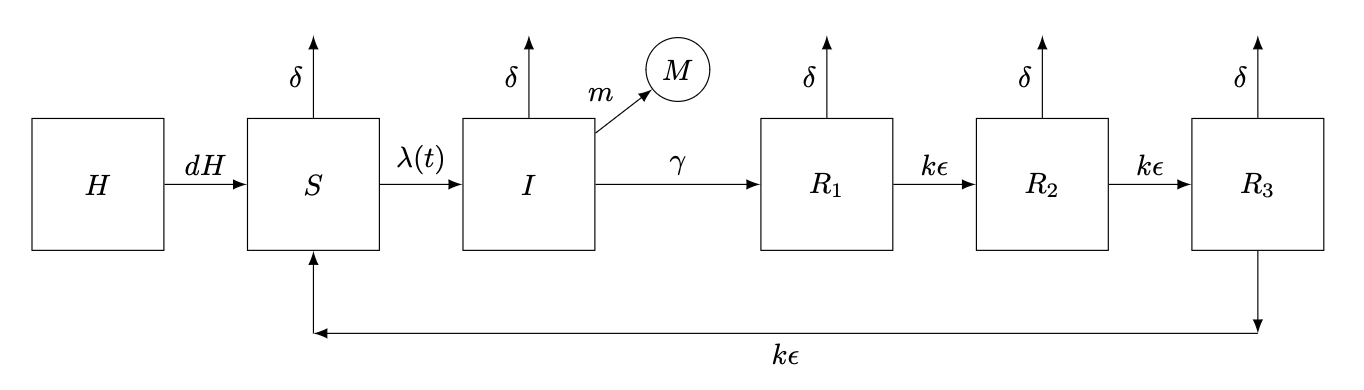
\includegraphics[scale=0.5]{imgs/dacca.png}
        \caption{Illustration of SIR model from \cite{king08}.}
        \label{fig:sir}
    \end{figure}
    
    \begin{itemize}
        \item Dhaka model from \cite{king08}, also used in \cite{ionides15} to benchmark IF2.
        \item \pause Stochastic SIR compartmental model with transition uncertainty driven by Brownian motion.
        \item \pause Force of infection $\lambda(t)$ modeled with splines for seasonality, etc.
    \end{itemize}
    
        %\item \pause Population $H(t)$ divided into:
        %\begin{itemize}
        %    \item \pause Susceptible compartment $S(t)$.
        %    \item \pause Infected compartment $I(t)$.
        %    \item \pause Three ($k=3$) recovered compartments $R_1(t), ..., R_k(t)$ denoting varying degrees of cholera immunity.
        %\end{itemize}
        %\item \pause $M(t)$ denotes the cholera deaths in each month.
\end{frame}

\begin{frame}{Results}
    
    \begin{table}[h!]
        \centering
        \begin{tabular}{||c c c||} 
         \hline
         Method & Best Log-Likelihood & Rank \\ [0.5ex] 
         \hline\hline
         IFAD-0.97 & $\textbf{-3750.21}$ & 1\\
         IFAD-0 & $-3752.17$ & 2\\
         IFAD-1 & $-3754.63$ & 3\\
         IF2 (Ours) & -3764.10 & 4\\
         IF2 (\cite{ionides15}) & -3768.63 & 5\\ 
         MOP-1 Alone (100 searches) & -3797.38 & 6\\
         \hline

        \end{tabular}
        \caption{\\
        -- IFAD performs the best among all methods, finding the MLE. \\
        -- Our implementation of IF2 outperforms that of \cite{ionides15} but underperforms IFAD.}
        \label{table:mle}
    \end{table}
    
    \begin{itemize}
        \item Benchmarked IFAD against IF2 on a challenging global search problem. 
        \item \pause Performed 44 searches each. 
    \end{itemize}
    
\end{frame}

\begin{frame}{Results}
    
\begin{figure}[htbp!]
    \centering
    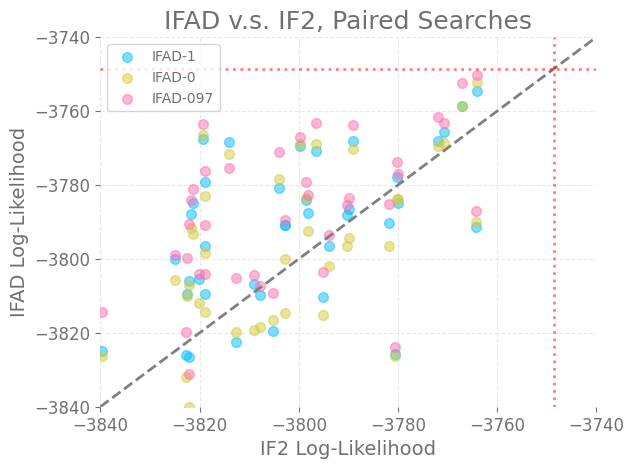
\includegraphics[scale=0.37]{imgs/095/pairs.png}
    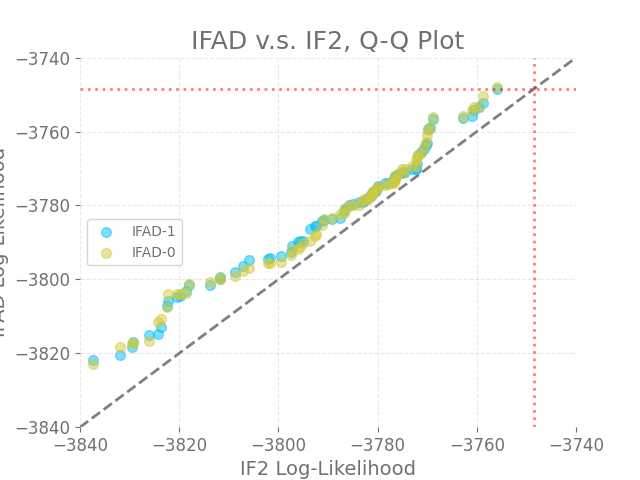
\includegraphics[scale=0.37]{imgs/095/qq.png}
    \caption{\\
    --\textbf{Left:} Paired searches from the same starting point. \\
    --\textbf{Right:} Q-Q plot of ranked IFAD searches against ranked IF2 searches. \\
    -- IFAD has the edge and manages to find the MLE.\\
    -- No IF2 search successfully gets within 7 log-likelihood units of it.}
    \label{fig:scatter}
\end{figure}
\end{frame}

\begin{frame}{Results}
    
\begin{figure}[H]
    \centering
    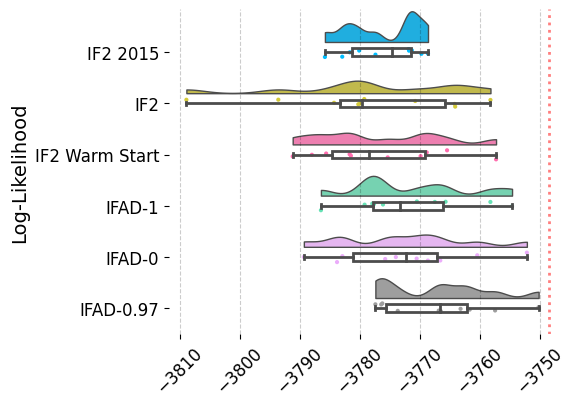
\includegraphics[scale=0.28]{imgs/095/boxplot.png}
    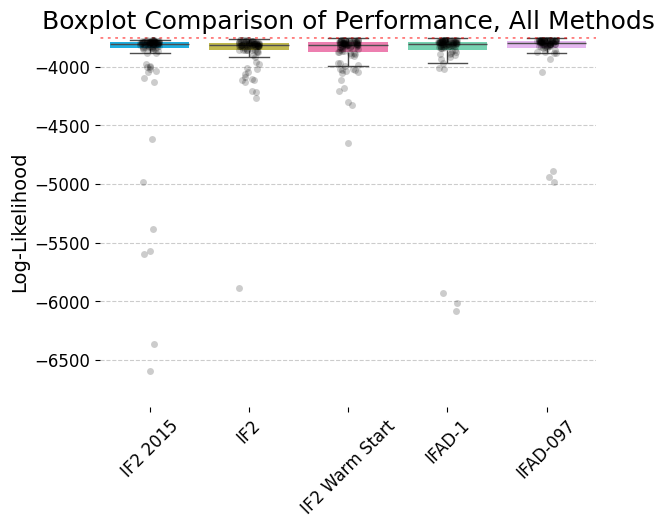
\includegraphics[scale=0.31]{imgs/095/boxplotall.png}
    \caption{\\
    -- \textbf{Left:} Results of best run out of every ten runs, simulating procedure of running a few searches and choosing the best one. \\
    -- \textbf{Right:} MOP alone drastically underperforms all other methods, failing to get close to the MLE. \\
    -- IF2 warm-start necessary in challenging nonconvex and noisy problems.}
    \label{fig:boxplot-search}
\end{figure}

\end{frame}

\begin{frame}{Results}
\begin{figure}[htbp!]
    \centering
    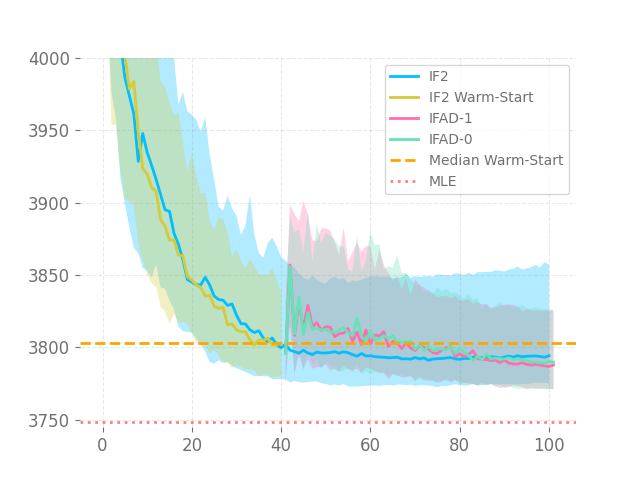
\includegraphics[scale=0.5]{imgs/095/optim.png}
    \caption{\\
    -- Solid lines depict the median negative log-likelihood at each iteration.\\
    -- Shaded area depicts the best search at any iteration and the 80\% percentile.}
    \label{fig:optim}
\end{figure}
%-- While running 60 more iterations of IF2 improves upon the median warm-start, doing so ultimately underperforms IFAD -- IFAD has better tail control and successfully reaches the MLE. The initial loss in log-likelihood upon transitioning from IF2 to MOP seems to help with escaping local minima. 
\end{frame}

\begin{frame}{Results}
    
\begin{figure}[u!]
    \centering
    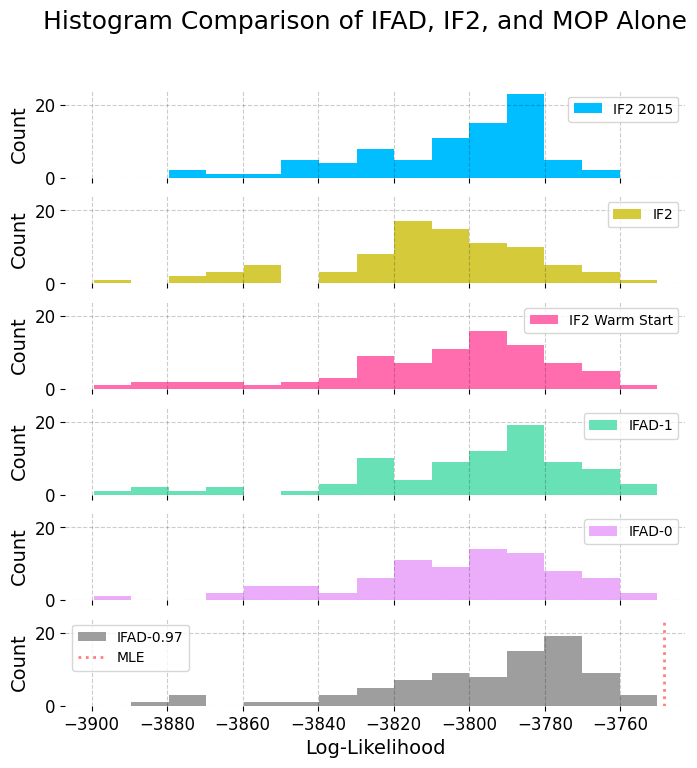
\includegraphics[scale=0.35]{imgs/095/hist.png}
    \caption{Histogram comparison of IFAD, IF2, and MOP alone. Right is better.}
    \label{fig:hist-all}
\end{figure}
\end{frame}

\begin{frame}{Takeaways}
    \begin{enumerate}
        \item IF2 converges quickly to a neighborhood of the MLE but fails to find the MLE.
        \item \pause Gradient steps perform better at fine-grained refinement.
        \item \pause Performing gradient steps alone without a warm-start leads to the search getting stuck in local minima and saddle points.
        \item \pause IFAD combines the best of IF2 and MOP, approaching the MLE quickly and successfully performing refinement -- even on a very difficult global search problem.
    \end{enumerate}
\end{frame}

\section{Conclusions and Future Work}

\begin{frame}{Conclusion}
    \begin{itemize}
        \item New theoretical framework/algorithm/gradient estimator that encompasses a few existing gradient estimates.
        \item \pause Promising hybrid algorithm that warm-starts gradient descent (using this estimator) with IF2.
        \item \pause Outperforms IF2 on Dhaka cholera model of \cite{king15}.
    \end{itemize}
\end{frame}


\begin{frame}{Future Work}
    \begin{itemize}
        \item MOP-$\alpha$ cannot handle discrete latent states. Maybe likelihood ratios can get around this.
        \item \pause Convergence rate of IF2 not known, conjecture similar behavior to SGD. 
        \item \pause Only gradient descent explored, other methods like Newton's method, ADAM, L-BFGS, etc. may perform better.
        \item \pause Extensions to panel and spatiotemporal data, e.g. with a block particle filter in the lens of \cite{ionides22} and \cite{ning23}.
        \item \pause Python counterpart to the popular \texttt{pomp} R package by \citet{king16, king2017pompmanual}.
    \end{itemize}
\end{frame}


\bibliographystyle{apalike}
\bibliography{mop/bib-ifad, mop/bib-ref}

\appendix
\section{Appendix}


\begin{frame}{Previous Work}

    
    \begin{itemize}
        \item \cite{poyiadjis11}, particle approximation of the score. \pause \\ \cite{scibior21}: AD + "stop-gradient trick". 
        \item 
        \pause \cite{blei2018vsmc}, backpropagate through vanilla particle filter.
        \item 
        \pause \cite{corenflos21}, optimal transport resampling.
        \item 
        \pause \cite{singh22}, fixed-lag smoothing.
    \end{itemize}
\end{frame}

\begin{frame}{Previous Work: Issues}
    \begin{itemize}
        \item Not (yet) compatible with desire for simulation-based inference.
        \begin{itemize}
            \item \pause Need modifications to use the bootstrap filter.
            \item \pause Sometimes special cases needed, e.g. transitions factoring into a policy and deterministic model (\cite{singh22}).
        \end{itemize}
        \item \pause Computationally expensive, quadratic in number of particles.
        \begin{itemize}
            \item \pause Optimal transport resampling (\cite{corenflos21}), marginal particle filters (\cite{scibior21}).
        \end{itemize}
        \item \pause High variance, or asymptotically biased.
        \begin{itemize}
            \item \pause Either one drops resampling terms and accepts asymptotic bias (\cite{blei2018vsmc}), or has variance quadratic in horizon (\cite{poyiadjis11}, \cite{scibior21})
        \end{itemize}
    \end{itemize}
\end{frame}

\begin{frame}{(Improved) Iterated Filtering (\cite{ionides15})}
    \begin{itemize}
        \item Only (practical) full-information, frequentist method of parameter estimation in POMPs that does not need transition densities. 
        \begin{itemize}
            \item \pause Each particle has its own set of parameters.
            \item \pause Particle parameters perturbed at every timestep.
            \item \pause Parameters resampled with their particles according to likelihood.
        \end{itemize}
        \item \pause Treats parameters as augmentations of the state space, evolving according to a random walk.
        \item \pause \textbf{Consistent estimates} via viewing this as a sequential Bayes map on the parameter distribution.
    \end{itemize}
\end{frame}

\begin{frame}{When Does IF2 Struggle?}

\begin{itemize}
    \item \textbf{IF2 is great at approaching the MLE quickly!}
    \item \pause Performs parameter updates at every timestep, so it does not need to wait to filter through the entire trajectory before each update.
    \item \pause \textbf{But struggles at squeezing out the last few units of log-likelihood.}
    \begin{itemize}
        \item \pause Especially true in highly nonlinear, nonconvex, and noisy settings, e.g. \textbf{disease models}. 
    \end{itemize}
\end{itemize}

\end{frame}

\begin{frame}{Assumptions}
        
    \begin{aspt}[Smooth Neighborhood]
    \label{assump:smooth-nbhd}
    There exists a neighborhood $\mathcal{N}(\phi)$ around any $\phi \in \Theta$ where for all $\theta \in \mathcal{N}(\phi)$ and almost every $\omega \in \Omega$, the Monte Carlo estimate of the likelihood at $\theta \in \mathcal{N}(\phi)$ with the system evolving according to $\phi$ conditional on $\omega$, $\hat\lik(\theta,\phi,\omega, J)$, is twice differentiable in $\theta$. 
    \end{aspt}

    \begin{itemize}
        \item \pause \textbf{Justification:} For suitably nearby $\theta$ and $\phi$, the resampling indices for $\hat\lik(\theta,\phi,\omega, J)$ and $\hat\lik(\phi,\phi,\omega, J)$ are the same.
        \item \pause This eliminates any discontinuities from resampling.
        \item \pause For small enough $\mathcal{N}(\phi)$, the likelihood ratios are bounded. 
        \item \pause The likelihood only changes by a factor of the likelihood ratios, which are bounded and smooth in $\theta$ if the densities used in the calculation are. 
    \end{itemize}
    
\end{frame}

\begin{frame}{Assumptions}
    
    \begin{aspt}[Continuity of the Likelihood] $\ell(\theta)$ proper is continuous in a neighborhood $\left\{\theta: \ell(\theta)>\lambda_1\right\}$ for some $\lambda_1<\sup _{\varphi} \ell(\varphi)$.
    \end{aspt}
    \pause 
    \begin{aspt}[Bounded Measurement Model] There is an $\epsilon>0$ with $\epsilon^{-1}>f_{Y_n \mid X_n}\left(y_n{ }^* \mid x_n; \theta\right)>\epsilon$ for all $1 \leq n \leq N, x_n \in \gX$ and $\theta \in \Theta.$
    \end{aspt}
    \pause 
    \begin{aspt}[Locally Bounded Derivative]
    \label{assump:local-bounded-derivative}
    Let $\mathcal{M}$ be an open subset of $\Omega$. There exists some function $G(\theta)$ and a constant $G=\sup _{\theta \in \mathcal{N}} G(\theta)<\infty$ such that
        $$
        \|\nabla \ell(\theta, \phi, \omega, J)\|_2<G(\theta) \leq G<\infty
        $$
        for every $\phi \in \mathcal{M}, \theta$ in smooth neighborhood $\mathcal{N}(\phi)$, and almost every $\omega \in \Omega$.
    \end{aspt}
\end{frame}


\begin{frame}{Algorithm: Measurement Off-Policy, MOP-$\alpha$}
    \begin{figure}
        \centering
        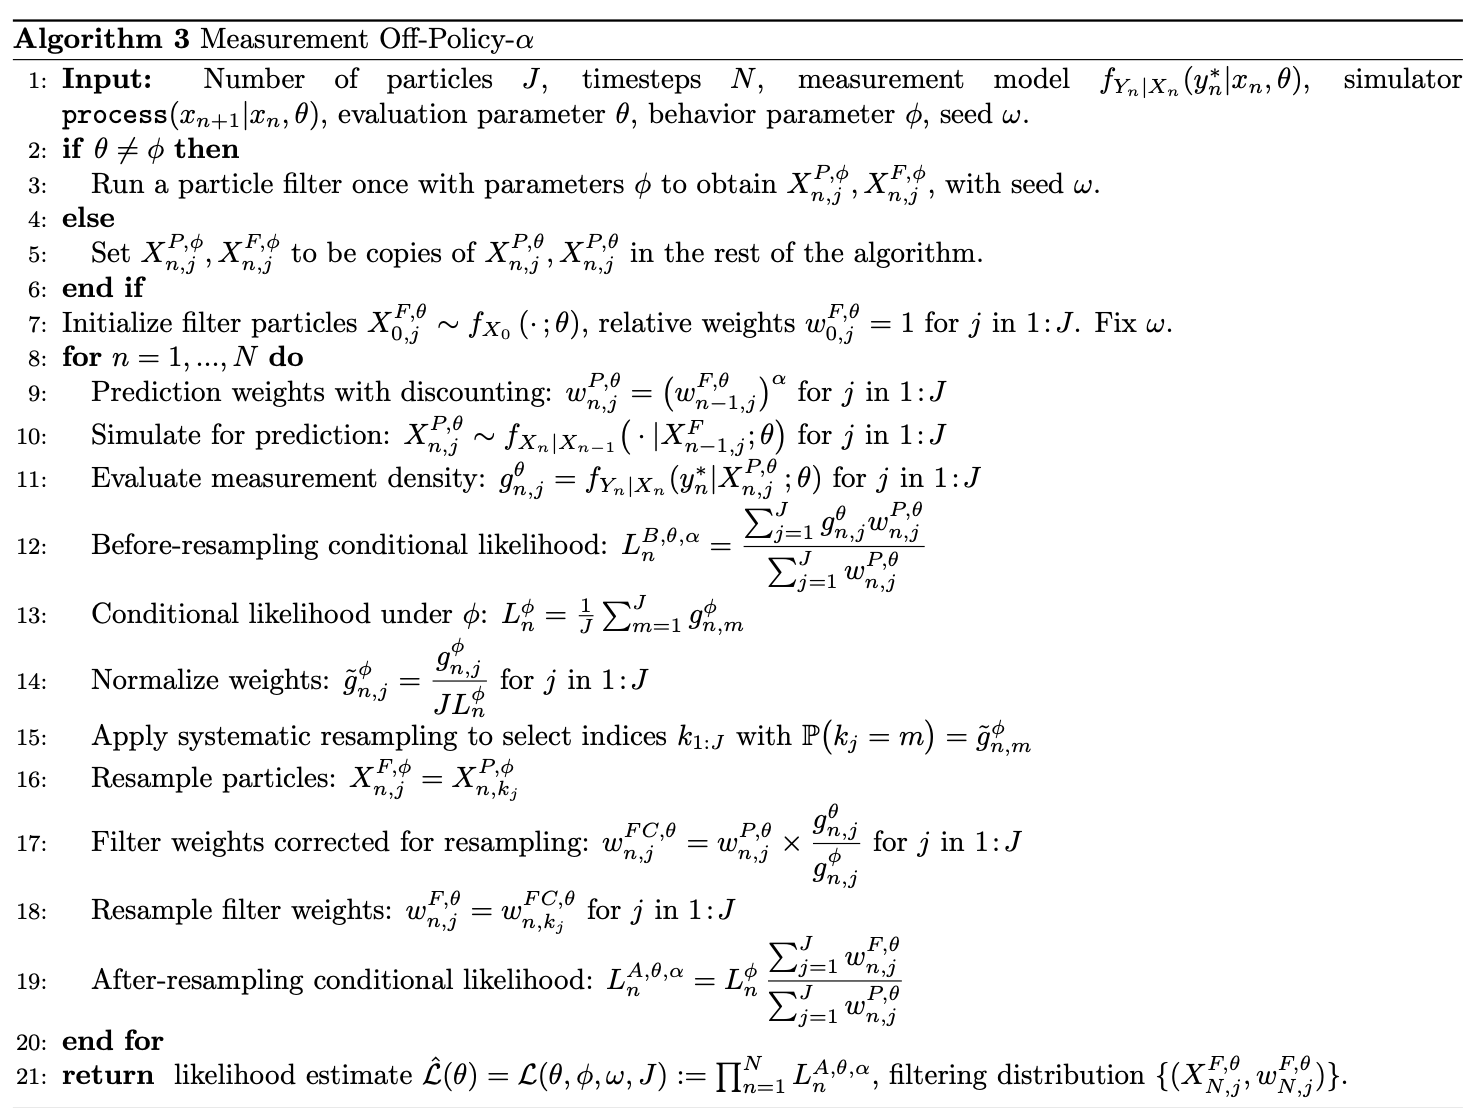
\includegraphics[scale=0.4]{imgs/mop.png}
        \caption{MOP-$\alpha$ algorithm.}
        \label{fig:mop}
    \end{figure}
\end{frame}


\begin{frame}{Why did we bother with this?}
    \begin{itemize}
        \item Lets us work with only a differentiable simulator.
        \item \pause Discounting parameter $\alpha$ helps with a bias-variance tradeoff (explained later). 
        \item \pause Gradients returned by the likelihood estimate $$\hat{\lik}(\theta) := \prod_{n=1}^N L_n^{A,\theta,\alpha} = L_n^\phi \, \frac{\sum_{j=1}^J w^{F,\theta}_{n,j}}{\sum_{j=1}^J  w^{P,\theta}_{n,j}}$$ have nice properties.
    \end{itemize}
\end{frame}


\begin{frame}{Iterated Filtering with Automatic Differentiation (IFAD)}
    \begin{figure}
        \centering
        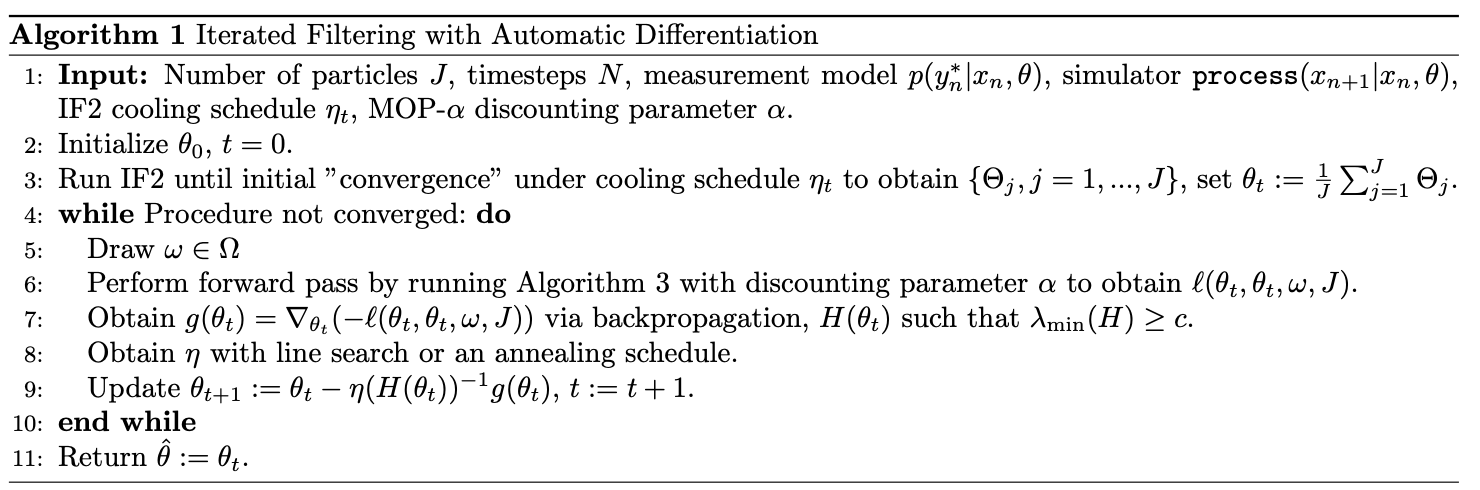
\includegraphics[scale=0.45]{imgs/ifad.png}
        \caption{Warm-starting first/second order iterative optimization with IF2.}
        \label{fig:ifad}
    \end{figure}
\end{frame}


\begin{frame}{Why does this help?}
    \begin{itemize}
        \item IF2 converges quickly, but struggles with last few log-likelihood units. 
        \item \pause Gradient descent gets stuck in saddle points and poor local minima when the likelihood is nonconvex. 
        \item \pause Warm-starting gradient methods with IF2:
        \begin{itemize}
            \item \pause Under regularity conditions, the likelihood is well-behaved near the MLE.
            \item \pause Issues with saddle points and local minima alleviated. 
        \end{itemize}
        \item \pause Combining these two lets us enjoy the best of both worlds.
    \end{itemize}
\end{frame}

\begin{frame}{Convergence Analysis}

    Guarantee currently only holds for IFAD-1, as it forms a particle approximation of the score as in \cite{poyiadjis11}.
    \begin{itemize}
        \item \pause Can be extended if the bias for the gradient estimate given by MOP-$\alpha$ for $\alpha < 1$ is small enough.
        \item \pause e.g. $\alpha$ close to 1, or $y_{n+1:N}^*$ uninformative of current state $x_n$ given past and current measurements $y_{0:n}^*$.
        \item \pause Otherwise, need to handle biased gradient descent.
    \end{itemize}

\end{frame}




\begin{frame}{Cholera in Bangladesh}
    The \textbf{transition dynamics} follow this series of stochastic differential equations driven by Brownian motion:
    \begin{align*}
        d S&=\left(k \epsilon R_k+\delta(S-H)-\lambda(t) S\right) d t+d H-(\sigma S I / H) d B, \\ 
        d I&=\left(\lambda(t) S-(m+\delta+\gamma) I\right) d t+(\sigma S I / P) d B, \\ 
        d R_1&=\left(\gamma I-(k \epsilon+\delta) R_1\right) d t, \\ 
        \vdots \\ 
        d R_k&=\left(k \epsilon R_{k-1}-(k \epsilon+\delta) R_k\right) d t,
    \end{align*}
\end{frame}

\begin{frame}{Cholera in Bangladesh}
The \textbf{force of infection}, $\lambda(t)$, is modeled by splines $s_j$, 
    \begin{equation*}
        \lambda(t)=\exp \left\{\beta_{\text {trend }}\left(t-t_0\right)+\sum_{j=1}^{6} \beta_j s_j(t)\right\}(I / P) + \exp \left\{\sum_{j=1}^{6} \omega_j s_j(t)\right\},
    \end{equation*}
    where
    \begin{itemize}
        \item \pause $\beta_j$ model seasonality in the force of infection.
        \item \pause $\beta_{\text{trend}}$ models the trend in the force of infection.
        \item \pause $\omega_j$ represent seasonality of a non-human environmental reservoir of disease.
    \end{itemize}
    
\end{frame}

\begin{frame}{Cholera in Bangladesh}
    The \textbf{measurement model} for observed monthly cholera deaths is given by 
    \begin{equation*}
        Y_n \sim \gN(M_n, \tau^2M_n^2),
    \end{equation*}
    where $M_n$ is the true number of cholera deaths in that month.
\end{frame}

\end{document}

